\documentclass[12pt, a4paper]{article}

\usepackage[slovene, english]{babel}
\usepackage[utf8]{inputenc}
\usepackage{amsmath, amsfonts}
\usepackage{url}
\usepackage{graphicx}
%\usepackage{tikz}
\usepackage{textpos}
\usepackage{wrapfig}
\usepackage{amsthm}
\usepackage{xparse}
\usepackage{interval}

%\usepackage{enumitem}

\setlength{\parskip}{0.5em}

\usepackage{graphicx}
\graphicspath{{figures}}

\newtheorem{izrek}{Izrek}
\newtheorem{trditev}{Trditev}
\newtheorem{lema}{Lema}
\newtheorem{definicija}{Definicija}
\newtheorem{pos}{Posledica}
\newtheorem{primer}{Primer}

\newcommand{\R}{\mathbb R}
\newcommand{\N}{\mathbb N}
\newcommand{\Z}{\mathbb Z}
\newcommand{\C}{\mathbb C}
\newcommand{\Q}{\mathbb Q}

\renewcommand{\mod}{\operatorname{mod}}

\title{Monochromatic crossings in the square}
\date{10.1.2023}
\author{Nino Cajnkar, Nika Pavlič}



\begin{document}
	\selectlanguage{slovene}
	\maketitle
	\section{Opis problema}
	Naj bo $P$ množica enakomernih naključnih $n$ točk v kvadratu (s stranico dolžine 1). Vsak par točk med seboj povežemo s povezavo in dobimo poln graf z $n$ vozlišči. Za množico kotov $\left[{a,b}\right]$ pobarvamo povezavo rdeče, če je kot, ki ga oklepa povezavo z $x$-osjo vsebovan v $\left[{a,b}\right]$, sicer pa jo pobarvamo z modro. V nalogi nas zanima število monokromatskih presečišč (to so taka presečišča katerih definirajoči povezave sta obe enake barve) in bikromatskih presečišč (definirajoči povezavi sta različne barve). Zanima nas, kako je to odvisno od velikosti intervala $\left[{a,b}\right]$, predvsem pri katerih intervalih je število bikromatskih vozlišč največje. \\
	Nadalje nas je zanimalo, kako se stvari spremenijo, če so točke enakomerno naključno porazdeljene v enotskem krogu. \\
	Kot dodaten problem sva si zastavila vprašanje, kaj pa se zgodi, če namesto kotov opazujemo dolžine povezav? Tukaj se problem malenkost spremeni, saj iščemo tak interval $\left[{a,b}\right]; a,b \in \left[0,\sqrt{2}\right]$ kjer je število monokromatskih vozlišč največje. Enako nas zanima tudi za enotski krog.
	\section{Podatki}
	Podatke sva generirala s pomočjo ukaza \texttt{rpoint} iz knjižnice \texttt{spatstat}, ki generira enakomerne naključne točke, v najinem primeru za kvadrat z dolžino stranice 1. Odločila sva se, da zaradi dolgega časa izvajanja programa pri višjem številu vozlišč obravnavava problem do 50 vozlišč. Tako sva generirala 45 vektorjev točk, sestavljenih iz $X$ in $Y$ koordinate in jih zapisala v datoteko tipa \texttt{.json} za lažji dostop v kasnejših delih. \\
	Generirane točke sva nato prebrala iz shranjene \texttt{.json} datoteke in s funkcijo \texttt{poln\_graf} vsak par točk med seboj povezala in dobila 45 polnih grafov z od 5 vozlišč in do 50 vozlišč. \\
	Sedaj sva morala najti vsa presečišča med povezavami v grafu, pri čemer sva si pomagala s pravilom levega zavoja.
	\begin{definicija}
		\textbf{Pravilo levega zavoja:} Naj bodo $P_1=(x_1,y_1),P_2=(x_2,y_2),P_3=(x_3,y_3)$ in $P_4=(x_4,y_4)$ točke v koordinatnem sistemu in naj bo $p$ daljica, ki povezuje $P_1$ in $P_2$ ter $r$ daljica, ki povezuje $P_3$ in $P_4$. Definirajmo \textbf{levi zavoj}
		$$Z(P_1,P_2,P_3)=\begin{vmatrix}
			1 & a_{x_1} & a_{y_1}\\ 
			1 & a_{x_2} & a_{y_2}\\
			1 & a_{x_3} & a_{y_3} 
		\end{vmatrix} > 0
	\Leftrightarrow (P_1,P_2,P_3) \text{ je levi zavoj.}$$
	Dalje, daljici $p$ in $r$ se sekata natanko tedaj, ko velja
	$$Z(P_1,P_2,P_3) \times Z(P_1,P_2,P_4) \leq 0 \wedge \\ 
	Z(P_3,P_4,P_1)\times Z(P_3,P_4,P_2)\leq 0$$
	\end{definicija}
	\noindent Generiranje točk v krogu se malenkost razlikuje in sicer sva si pomagala s še enim ukazom iz knjižnice \texttt{statspat} in sicer \texttt{runifdisc}. Nadaljni postopek generiranja povezav je enak kot v kvadratu. 
	\noindent S funkcijo \texttt{presecisca} sva tako poiskala vsa presečišča in jih zapisala v \texttt{data frame}, za vsako presečišče sva še izračunala naklon povezav, ki ga definirajo ter njihovo dolžino. Postopek ugotavljanja presečišč je enak tudi za točke v enotskem krogu. Podatke o presečiščih za krog in kvadrat sva nato spet prepisala v \texttt{.json} datoteko za kasnejši lažji dostop. \\
	\begin{figure}[h!]
		\caption{Poln graf za enakomerno naključno generiranih 20 točk v kvadratu}
		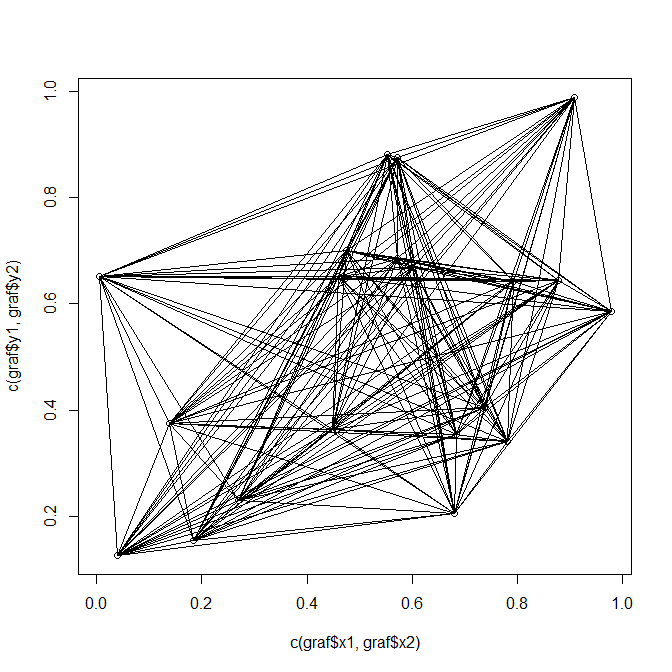
\includegraphics[scale=0.6]{graf_20}
		\centering
	\end{figure}
	\begin{figure}[h!]
		\caption{Poln graf za enakomerno naključno generiranih 20 točk v krogu}
		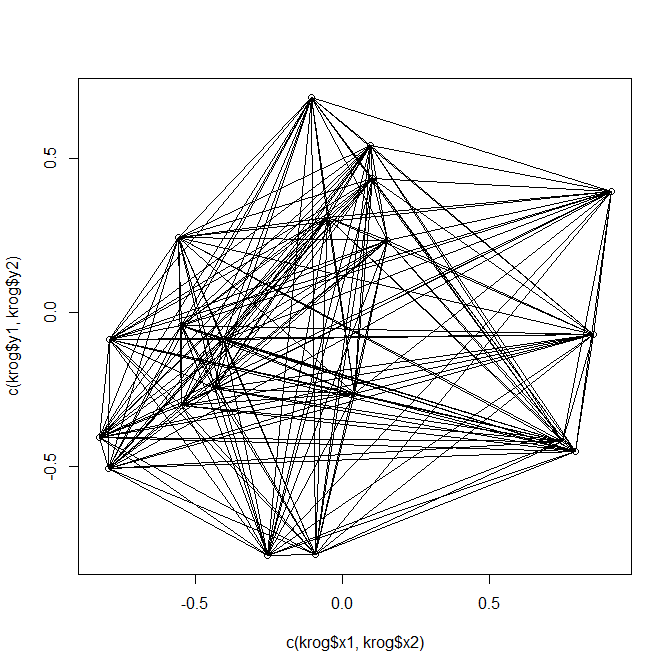
\includegraphics[scale=0.6]{krog_20}
		\centering
	\end{figure}
	\section{Reševanje problema}
	\subsection{Barvanje točk v kvadratu glede na interval kotov}
	V datotekah tipa \texttt{.json} imamo sedaj shranjena presečišča, naklone in dolžine povezav, sedaj pa moramo povezave še pobarvati. In sicer to naredimo s pomočjo funkcije \texttt{barvanje}, ki pobarva povezave rdeče, če je njen naklon vsebovan v intervalu $\left[{a,b}\right]; \ a,b \in \left[{-\pi/2,\pi/2}\right]$ in modro sicer. \\
	Dalje definiramo dve funkciji \texttt{racunanje\_kotov}, ki sprejme podatke o presečiščih in za intervale $\left[{a,b}\right]$, kjer $a \in \left[{-\pi/2, \pi/2}\right]$ s korakom $\pi/20$ in $b \in \left[{a, \pi/2}\right]$ s korakom $\pi/20$, najprej vsako povezavo obarva rdeče ali modro s funkcijo \texttt{barvanje}, nato pa vsakemu presečišču priredi vrednost \textit{mono} ali \textit{bi}, glede na to ali je presečišče monokromatsko ali bikromatsko. Funkcija vrne \texttt{data frame} intervalov preverjanja ter število monokromatskih presečišč v stolpcu \texttt{obarvanost}. Funkcija \texttt{racunanje\_min\_kotov} vrne največji tak interval, v katerem je število monokromatskih presečišč najmanjše. \\
	Ta funkcija je uporabljena za izračun intervalov ter najmanjšega števila monokromatskih presečišč vseh polnih grafov, katere zaporedoma prebere iz datotek \texttt{.json}, ter vrne spremenljivko \texttt{skupni\_min}, v kateri so združeni ti koti ter števila. \\
	Izračunamo še frekvenčni diagram, v katerem zabeležimo začetke intervalov ter število minimumov, ki se znotraj njih pojavijo. To shranimo v spremenljivko \texttt{frekvencni}. Za manjše število vozlišč (kar obravnavamo v našem primeru) opazimo, da največ minimumov najdemo na intervalu $\left[{-\pi/4, -7\pi/20}\right]$ oziroma $\left[{-\pi/4, -\pi/10}\right]$. Lahko bi rezultate še nadalje analizirali, na primer kateri znani porazdelitvi se najbolje prilegajo ter izračunali intervale zaupanja, vendar rezultati ne bi bili zelo natančni zaradi manjšega vzorca. \newpage
	\begin{figure}[h!]
		\caption{Frekvenčna analiza intervalov kotov, kjer se pojavijo minimumi monokromatskih presečišč generiranih točk v kvadratu}
		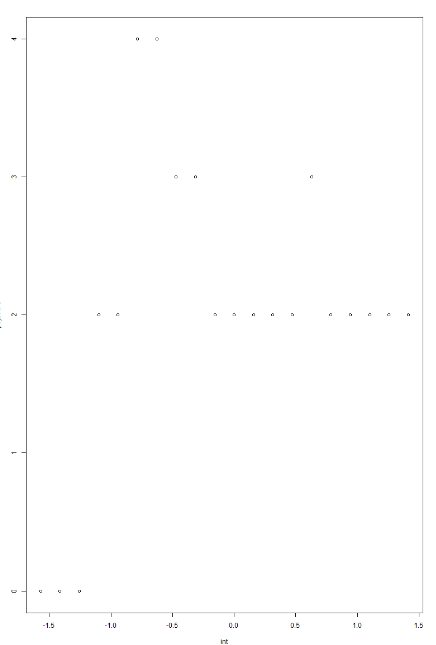
\includegraphics[scale=0.6]{frekvencni}
		\centering
	\end{figure}
	
	\subsection{Barvanje točk v krogu glede na interval kotov}
	Postopek barvanja generiranih polnih grafov iz točk znotraj enotskega kroga je praktično identičen, vendar dobimo drugačne rezultate. Meje najboljših  intervalov so precej premaknjene v pozitivno smer, z največ najdbami minimumov na intervalu $\left[{-\pi/10, \pi/10}\right]$ oziroma $\left[{-\pi/5, \pi/10}\right]$. Rezultati so malenkost manj zanesljivi zaradi osamelca, kar pa lahko pripišemo naključnosti generiranja točk in posledično generiranih grafov, kar bi nadaljna analiza najverjetneje tudi potrdila.
	\begin{figure}[h!]
	\caption{Frekvenčna analiza intervalov kotov, kjer se pojavijo minimumi monokromatskih presečišč generiranih točk v krogu}
	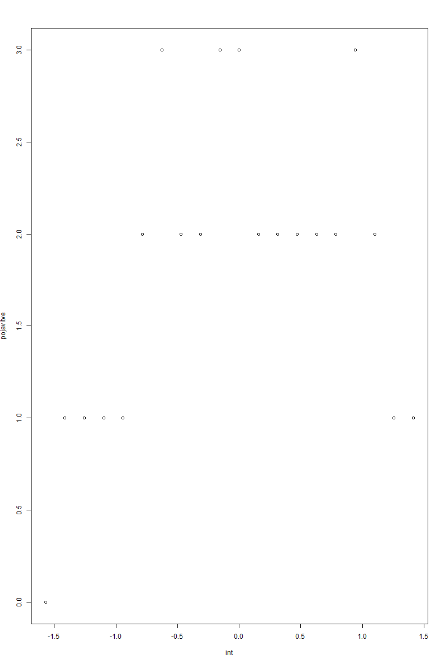
\includegraphics[scale=0.6]{frekvencni_krog}
	\centering
	\end{figure}
	\subsection{Barvanje točk v kvadratu glede na intervale dolžin povezav}
	Tukaj se naloga razlikuje od prejšnje, saj iščemo maksimalno število monokromatskih presečišč. \\
	Tako kot v primeru gledanja kotov imamo v datotekah tipa \texttt{.json} shranjena presečišča, naklone in dolžine povezav, sedaj pa moramo povezave še pobarvati. In sicer to naredimo s pomočjo funkcije \texttt{barvanje\_dol}, ki pobarva povezave rdeče, če je njena dolžina vsebovana v intervalu $\left[{a,b}\right]; \ a,b \in \left[{0,\sqrt{2}}\right]$ in modro sicer. \\
	Dalje definiramo dve funkciji \texttt{racunanje\_dolzin}, ki sprejme podatke o presečiščih in za intervale $\left[{a,b}\right]$, kjer $a \in \left[{0, \sqrt{2}}\right]$ s korakom $\sqrt{2}/20$ in $b \in \left[{a, \sqrt{2}}\right]$ s korakom $\sqrt{2}/20$, najprej vsako povezavo obarva rdeče ali modro s funkcijo \texttt{barvanje\_dol}, nato pa vsakemu presečišču priredi vrednost \textit{mono} ali \textit{bi}, glede na to ali je presečišče monokromatsko ali bikromatsko. Funkcija vrne \texttt{data frame} intervalov preverjanja ter število monokromatskih presečišč v stolpcu \texttt{obarvanost}. Funkcija \texttt{racunanje\_max\_dolzin} vrne največji tak interval, v katerem je število monokromatskih presečišč največje. \\
	Ta funkcija je uporabljena za izračun intervalov ter največjega števila monokromatskih presečišč vseh polnih grafov, katere zaporedoma prebere iz datotek \texttt{.json}, ter vrne spremenljivko \texttt{skupni\_max\_dolzin}, v kateri so združene te dolžine ter števila. \\
	Izračunamo še frekvenčni diagram, v katerem zabeležimo začetke intervalov ter število maksimumov, ki se znotraj njih pojavijo. To shranimo v spremenljivko \texttt{frekvencni\_dolzin}. Za manjše število vozlišč (kar obravnavamo v našem primeru) opazimo, da največ maksimumov najdemo na intervalu $\left[{\sqrt{2}/5, 2\sqrt{2}/5}\right]$. Intervali so precej bolj enakomerno razporejeni kot pri obravnavi intervalov kotov.
	\begin{figure}[h!]
		\caption{Frekvenčna analiza intervalov dolžin, kjer se pojavijo maksimumi monokromatskih presečišč generiranih točk v kvadratu}
		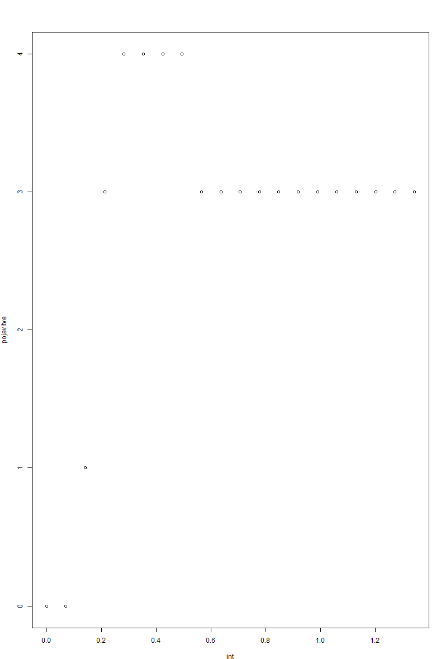
\includegraphics[scale=0.6]{frekvencni_dolzin}
		\centering
	\end{figure}
	\subsection{Barvanje točk v krogu glede na intervale dolžin povezav}
	Postopek barvanja generiranih polnih grafov iz točk znotraj enotskega kroga je podoben, le da se tukaj možne dolžine povezav razlikujejo, saj je maksimalna možna razdalja enaka premeru enotskega kroga, torej 2. Barvamo torej glede na intervale $\left[{a,b}\right]; \ a,b \in \left[{0,2}\right]$ s korakom $0.1$. \\
	Meje najboljših  intervalov so precej premaknjene v pozitivno smer, z največ najdbami maksimumov na intervalu $\left[{0.3, 0.7}\right]$ oziroma $\left[{0.3, 1.0}\right]$. Rezultati so tudi tukaj malenkost manj zanesljivi kot pri analizi dolžin v kvadratu, kar pa lahko pripišemo naključnosti generiranja točk in posledično generiranih grafov, kar bi nadaljna analiza najverjetneje tudi potrdila.
	\begin{figure}[h!]
		\caption{Frekvenčna analiza intervalov dolžin, kjer se pojavijo maksimumi monokromatskih presečišč generiranih točk v krogu}
		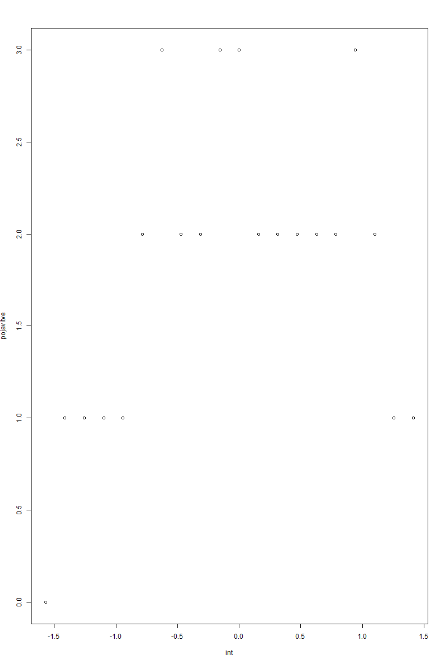
\includegraphics[scale=0.6]{frekvencni_krog}
		\centering
	\end{figure}
	\section{Zaključek}
	Za rešitve je bilo generiranih 45 polnih grafov pri vsakem podproblemu, izračunana ter obarvana so bila presečišča ter opravila se je analiza rezultatov. Za natančnejše rezultate bi bilo potrebno generirati ali večje število polnih grafov pri posameznih številih generiranih točk ter polni grafi z večjim številom vozlišč ter povezav. Odkrili smo, da se rezultati za točke generirane v kvadratu ter krogu razlikujejo, dalje bi bilo zanimivo analizirati tudi kako se stvari nadalje spreminjajo v večkotnikih, na primer da generiramo točke v trikotniku, petkotniku in poljubnem n kotniku. Možna naloga bi bila tudi primerjati razlike v rezultatih med kvadratom in krogu očrtanem kvadratu.
\end{document}